\documentclass{article}
\usepackage{amsmath}
\usepackage{amsthm}
\usepackage{amssymb}
\usepackage{amsfonts}
\usepackage{mathtools}
\usepackage{listings}
\title{MATH 620: Homework 5}
\author{Fernando}
\date{\today}
\begin{document}
\maketitle
\section*{Problem 1}
\subsection*{Part 1}
According to the definition we need that
\[
	\int u \phi' = -\int g \phi
\]
for every bump function $\phi$.

First we can see that $g\equiv 0$ on $(-\infty,0)$ because $u$ is constant
there. Same argument shows that $g\equiv 0$ on $(0,\infty)$, then
$g\equiv 0$, which means that $\int u \phi' = 0$ for all bump
functions $\phi$. But this is clearly not true because the fundamental theorem
of variations would imply that $u=0$. Another way to see that this is false is
taking a specific bump function, for example $e^{-1/(1-x^2)}$. According to
Wolfram Alpha its derivative looks like this:

\begin{center}
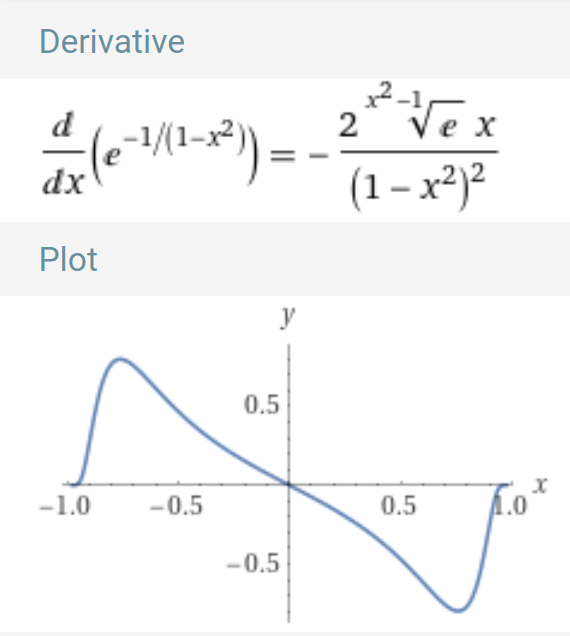
\includegraphics[width=0.5\textwidth]{bumpPrime.png}
\end{center}

Then multiplying by $u$ kills everything after 0 and multiplies by -1 the part
before 0. If we integrate that, the result is clearly not 0.
\subsection*{Part 2}
Following the suggestion we change to polar coordinates.
Then $u$ becomes:
\[
u(\theta)=\sin(\arctan(\tan(\theta)))=\begin{cases}
	\sin(\theta) \quad \text{for } -\frac{\pi}{2} < \theta < \frac{\pi}{2}\\
	-\sin(\theta) \quad \text{for } \frac{\pi}{2} < \theta < \frac{3\pi}{2}
\end{cases}.
\]
Intuitively the weak derivative should be
\[
g(\theta)=\begin{cases}
	\cos(\theta) \quad \text{for } -\frac{\pi}{2} < \theta < \frac{\pi}{2}\\
	-\cos(\theta) \quad \text{for } \frac{\pi}{2} < \theta < \frac{3\pi}{2}
\end{cases}.
\]
Now let's prove it. Let $B$ be the unit ball, then
\begin{align*}
	\int_{B}u\partial_{\theta}\phi &=\int_{-\frac{\pi}{2}}^{\frac{\pi}{2}} \int_0^1 \sin(\theta)\partial_\theta\phi drd\theta
		      -\int_{\frac{\pi}{2}}^{\frac{3\pi}{2}} \int_0^1 \sin(\theta)\partial_\theta\phi drd\theta\\
		      &=\int_0^1 \int_{-\frac{\pi}{2}}^{\frac{\pi}{2}} \sin(\theta)\partial_\theta\phi d\theta dr
		      -\int_0^1 \int_{\frac{\pi}{2}}^{\frac{3\pi}{2}} \sin(\theta)\partial_\theta\phi d\theta dr\\
		      &=\int_0^1 \int_{-\frac{\pi}{2}}^{\frac{\pi}{2}} \sin(\theta)\partial_\theta\phi d\theta dr
		      -\int_0^1 \int_{\frac{\pi}{2}}^{\frac{3\pi}{2}} \sin(\theta)\partial_\theta\phi d\theta dr\\
		      &=\int_0^1 \left( [\phi(r,\pi/2)+\phi(r,-\pi/2)]- \int_{-\frac{\pi}{2}}^{\frac{\pi}{2}} \cos(\theta)\phi d\theta \right) dr\\
		      &-\int_0^1 \left( [\phi(r,3\pi/2)+\phi(r,\pi/2)]- \int_{\frac{\pi}{2}}^{\frac{3\pi}{2}} \cos(\theta)\phi d\theta \right) dr\\
		      &=\int_0^1 \left[ \phi(r,-\pi/2)-\phi(r,3\pi/2) + \int_{\frac{\pi}{2}}^{\frac{3\pi}{2}} \cos(\theta)\phi d\theta - \int_{-\frac{\pi}{2}}^{\frac{\pi}{2}} \cos(\theta)\phi d\theta \right] dr\\
		      &=\int_0^1 \left(\int_{\frac{\pi}{2}}^{\frac{3\pi}{2}} \cos(\theta)\phi d\theta - \int_{-\frac{\pi}{2}}^{\frac{\pi}{2}} \cos(\theta)\phi d\theta \right) dr\\
		      &=-\left(\int_{-\frac{\pi}{2}}^{\frac{\pi}{2}} \int_0^1 \cos(\theta)\phi drd\theta
		        -\int_{\frac{\pi}{2}}^{\frac{3\pi}{2}} \int_0^1 \cos(\theta)\partial_\theta\phi drd\theta\right)\\
		      &=-\int_{B}g\phi.
\end{align*}
And analogously:
\begin{align*}
	\int_{B}u\partial_r\phi &=\int_{-\frac{\pi}{2}}^{\frac{\pi}{2}} \int_0^1 \sin(\theta)\partial_r\phi drd\theta
		      -\int_{\frac{\pi}{2}}^{\frac{3\pi}{2}} \int_0^1 \sin(\theta)\partial_r\phi drd\theta\\
		  &=\int_{-\frac{\pi}{2}}^{\frac{\pi}{2}} \sin(\theta)\int_0^1 \partial_r\phi drd\theta
		      -\int_{\frac{\pi}{2}}^{\frac{3\pi}{2}} \sin(\theta)\int_0^1 \partial_r\phi drd\theta\\
		  &=\int_{-\frac{\pi}{2}}^{\frac{\pi}{2}} \sin(\theta) \phi(0,\theta)d\theta
		      -\int_{\frac{\pi}{2}}^{\frac{3\pi}{2}} \sin(\theta)\phi(0,\theta) d\theta\\
		  &=\int_{-\frac{\pi}{2}}^{\frac{3\pi}{2}} \sin(\theta) (\phi(0,\theta)-\phi(0,\theta))d\theta\\
		  &=0.
\end{align*}
So the weak gradient IN THE POLAR COORDINATE SYSTEM is $(0,g(\theta))$. If we
wanted the weak gradient in $x,y$ coordinates we would need to go back, but we
can't just change variables because we would be ignoring the chain rule. Going
back would require a lot of messy calculations I believe, so I will leave this
expressed in the polar coordinate system.
\section*{Problem 2}
Let $\varphi$ be a linear functional. We have to prove that $\varphi$ is continuous
iff $\varphi$ is bounded.
\subsection*{Continuous $\implies$ Bounded}
By contradiction assume that there is a continuous and unbounded $\varphi$.
Then we can find a sequence $x_k$ such that $\varphi(x_k)>k$. And without loss
of generality we can assume $||x_k||_X=1$. Now consider the sequence
$\frac{x_k}{k}$. We can see that $||\frac{x_k}{k}||_X=1/k$, then $\frac{x_k}{k}
\to 0$, but $\varphi(\frac{x_k}{k})=\frac{1}{k}\varphi(x_k)>1$. So
$\varphi(\frac{x_k}{k}) \not \to 0$, which contradicts the hypothesis that
$\varphi$ is continuous.
\subsection*{Bounded $\implies$ Continuous}
Let $x_k \to x$ i.e. $||x_k-x||_X \to 0$. By hipothesis
\[
	|\varphi(x_k-x)|\leq c ||x_k-x||_X
\]
so $\varphi(x_k-x) \to 0$. Then by linearity $\varphi(x_k)\to \varphi(x)$.

\section*{Problem 3}
\subsection*{Part 1}
\subsubsection*{Linearity}
\begin{align*}
	\varphi(u+\lambda v) &= \int_\Omega a(x)(u+\lambda v)(x)dx\\
	         &= \int_\Omega a(x)u(x)dx + \lambda\int_\Omega a(x)v(x)dx\\
		 &= \varphi(u) + \lambda \varphi(v)
\end{align*}
\subsubsection*{Boundedness}
By H\"older's inequality we have
\[
	|\varphi(u)|=\bigg|\int_\Omega a(x)u(x)dx\bigg|\leq ||a||_{L^q}||u||_{L^p}
\]
So in this case our constant is $||a||_{L^q}$, which is finite by hypothesis.
\subsection*{Part 2}
Let's do a simple example. For simplicity we pick $p=q=2$ and $\Omega = [0,1]$.
Then we choose $a=\frac{1}{x^{0.75}}$. The functional that $u$ induces is
\[
	\varphi(u)=\int_0^1 \frac{u}{x^{0.75}}
\]
This functional is linear; however it is not bounded because if we consider the
$L_2$ function $u=\frac{1}{x^{0.25}}$ then $\varphi(u)=\int_0^1
\frac{1}{x}=\infty$. So this choice of $a$ does not give us a valid element of
the dual space.
\section*{Problem 4}
\section*{Problem 5}
\end{document}
